
\chapter{Trabajos Relacionados\label{chap:Trabajos-Relacionados}}

El enfoque propuesto es un proceso de aprendizaje de máquina que incluye
una herramienta para recolectar mediciones de performance en Android,
y otra herramienta para entrenar y evaluar modelos de predicción con
diferentes técnicas de aprendizaje automático. En este capítulo se
presentan trabajo relacionados, divididos en dos secciones. Primero,
en la sección \ref{sec:Herramientas-de-benchmarks-para-Android},
se describe un conjunto de herramientas para monitorear y realizar
pruebas de performance en Android. Luego, en la sección \ref{sec:Predicci=0000F3n-de-propiedades-no-funcionales-con-aprendizaje-de-m=0000E1quina},
se presentan algunos trabajos relacionados que también abordan el
problema de predicción de atributos no-funcionales con técnicas de
aprendizaje de máquina.


\section{Herramientas para Android\label{sec:Herramientas-de-benchmarks-para-Android}}

Las herramientas de monitoreo y pruebas de performance para Android
ofrecen a los desarrolladores la posibilidad de analizar los aspectos
no-funcionales de una aplicación Android arrojando datos numéricos
acerca de su desempeño y consumo de recursos. A continuación se describen
algunas de estas herramientas. 


\subsection*{Performance Monitors de Android \label{sub:Performance-Monitors-de-Android }}

Es una herramienta integrada en el ambiente de desarrollo \emph{Android
Studio}\footnote{\emph{https://developer.android.com/studio/profile/android-monitor.html}}
y cuenta con varias sub herramientas que monitorean y proveen información
en tiempo real sobre la aplicación. Los datos capturados se almacenan
en archivos para luego analizarlos en diferentes vistas. Pueden monitorearse
tanto aplicaciones en dispositivos reales conectados o simulados a
través de un emulador.

A través de cinco vistas diferentes se accede a la información sobre
la aplicación evaluada. \emph{LogCat} monitorea las excepciones y
mensajes de log emitidos por la aplicación y el sistema operativo,
útil para deputar la aplicación durante su desarrollo. Las restantes
vistas proveen un monitoreo del consumo de memoria, CPU, GPU y red
por parte de la aplicación.


\subsection*{Benchit\label{sub:Benchit}}

\emph{Benchit}\footnote{\emph{https://github.com/T-Spoon/Benchit}}
es una biblioteca Open Source implementada en lenguaje Java para realizar
mediciones de performance en Android. Benchit es rápido y sencillo
de usar, ya que permite analizar áreas de código para determinar el
tiempo de respuesta o latencia de la operación. Una forma sencilla
de utilizar esta librería es a través de iteraciones sobre una misma
sección de código. De esta forma, con cada iteración, la herramienta
va almacenando el tiempo de ejecución del código (diferencia entre
el tiempo de comienzo y tiempo de fin). Al término de las iteraciones,
se podrá extraer el promedio, rango y desviación estándar de las mediciones.
La herramienta, también provee la posibilidad de realizar comparaciones
de código mostrando los resultados de manera ordenada. Esta opción
es útil, por ejemplo, al momento de comparar el desempeño de distintos
algoritmos o porciones de código que realicen la misma acción de forma
diferente. 


\subsection*{Google Caliper \label{sub:Google-caliper}}

\emph{Google Caliper} es un framework open source para implementar,
ejecutar y visualizar resultados de microbenchmarks en aplicaciones
Java, aunque brinda soporte para proyectos Android. Los microbenchmarks
son mediciones realizadas a funciones simples como llamadas al kernel.
Caliper permite obtener diferentes medidas del código Java, principalmente
microbenchmarks, pero también tiene soporte para otros tipos de medidas
incluyendo memoria disponible, u otras medidas arbitrarias de dominio
específico como por ejemplo el radio de compresión. 


\subsection*{JMeter\label{sub:JMeter}}

\emph{Apache JMeter} es una herramienta Open Source implementada en
lenguaje Java para realizar pruebas de carga y rendimiento de una
variedad de servicios, con énfasis en aplicaciones y protocolos Web.
Apache JMeter se puede utilizar para simular un gran volumen de carga
en un servidor o grupo de servidores y probar su resistencia o analizar
el rendimiento general bajo diferentes tipos de carga. En un principio,
fue diseñada para realizar pruebas de rendimiento sobre aplicaciones
Web pero luego ha sido extendida a otras funciones para cubrir diferentes
categorías de testing, tal es el caso de los análisis de carga, de
funcionalidad, desempeño, regresión, entre otros. JMeter es una aplicación
de escritorio con una interfaz gráfica amigable para el usuario. Puede
ser ejecutada bajo cualquier entorno o estación que acepte la máquina
virtual de Java como es el caso de los sistemas operativos Windows,
Linux y Mac.

A grandes rasgos, la herramienta simula un grupo de usuarios que envían
peticiones a un servidor y retorna un conjunto de estadísticas sobre
el desempeño y funcionalidad por medio de gráficos, tablas, etc, tanto
sobre recursos estáticos y dinámicos. 

El cuadro \ref{tab:benchmarks-tools} presenta y compara las principales
características de las herramientas antes mencionadas.

\begin{table}[h]
\begin{centering}
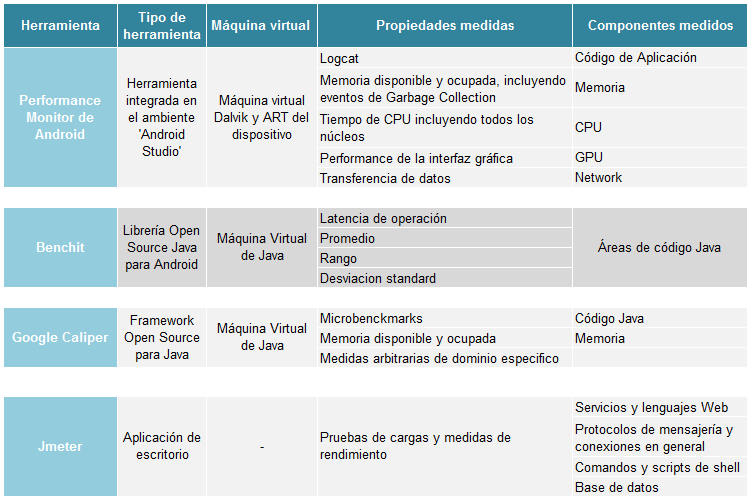
\includegraphics[scale=0.47]{images/benchmarks_tools}
\par\end{centering}

\caption{Información resumida de herramientas de pruebas de performance para
aplicaciones Android y servicios Web.}
\label{tab:benchmarks-tools}
\end{table}



\section{Predicción de propiedades no-funcionales con aprendizaje de máquina
\label{sec:Predicci=0000F3n-de-propiedades-no-funcionales-con-aprendizaje-de-m=0000E1quina}}

La predicción de propiedades no-funcionales ayuda a los arquitectos
de software en la evaluación de sus sistemas durante la etapa de diseño,
y a guiar las decisiones respecto a que componentes integrar a la
arquitectura del sistema de acuerdo a sus requerimientos de calidad.
Diferentes trabajos han recurrido al uso de técnicas de aprendizaje
de máquina para construir modelos de predicción de performance y otros
atributos de calidad dinámicos. En \citet{Hutter2014}se refieren
a estos modelos como modelos empíricos de performance (\emph{EPM}
por sus siglas en inglés) ya que requieren la recolección de mediciones
empíricas sobre los componentes. 

La principal aplicación de estos modelos probablemente es el problema
de selección de algoritmos, introducido en 1976 por John R. Rice \citep{Rice1976}.
Este problema consiste en seleccionar el algoritmo, o configuración
de algoritmo, de un portafolio de alternativas que minimice el tiempo
de respuesta, según la instancia de datos de entrada. La predicción
del tiempo de respuesta ha sido abordada con éxito usando técnicas
de aprendizaje supervisado, principalmente de regresión \citep{Hutter2014}.
En estos trabajos, los datos empíricos de entrenamiento son obtenidos
en contextos de ejecución controlados, para enfocarse en la correlación
entre la propiedad a predecir y las propiedades de los parámetros
de entrada del algoritmo. Una limitación de estos modelos es que no
generalizan la predicción de las propiedades de performance al contexto
de ejecución, es decir, no consideran características del dispositivo
y el ambiente de ejecución que influyen sobre el desempeño del componente,
como su capacidad de cómputo y la disponibilidad de recursos. 

Los modelos de predicción no sólo se utilizan para estimar el tiempo
de respuesta del desempeño de los componentes, sino también para estimar
otras propiedades. Por ejemplo, en \citet{Roberts07learnedmodels}
se proponen modelos para la predicción del tiempo de respuesta y para
la probabilidad de éxito de diferentes algoritmos de planeamiento
utilizando técnicas de aprendizaje de máquina incluidas en la librería
Weka. Para el aprendizaje fueron utilizados los resultados de 4726
instancias de problemas de planning ejecutadas sobre 28 algoritmos
de planeamiento conocidos. Por cada algoritmo y cada problema se registra
si un plan fue encontrado exitosamente o no, y el tiempo (en segundos)
requerido en completar la ejecución. A partir de esta información
se entrenan y evalúan modelos con diferentes técnicas de aprendizaje
supervisado. El trabajo presentado en \citet{Beveridge2009} también
analiza la precisión de distintos algoritmos, en este caso, para el
reconocimiento de rostros en imágenes, utilizando una técnica de regresión
lineal denominada GLMM, por Generalized Linear Mixed Models. 

Otros autores en \citet{Mersmann_anovel} predicen la optimalidad
o razón de aproximación de algoritmos para el problema del viajante
utilizando una técnica de regresión no lineal llamada \emph{MARS},
por sus siglas en inglés. El modelo \emph{MARS} se aplicó con éxito
para predecir la optimalidad del algoritmo de búsqueda local llamado
2-opt, independientemente del tamaño de la instancia del problema.
Se argumenta que es sencillo aplicar la misma metodología a otros
algoritmos y utilizar estos modelos para derivar una estrategia para
el problema de selección de algoritmos en el contexto del problema
del viajante.

La predicción de propiedades dinámicas de servicios Web, como su tiempo
de respuesta, y probabilidad de fallos, es más compleja de abordar
con respecto a algoritmos y componentes ejecutados localmente ya que
depende de factores propios de la infraestructura de red y el proveedor
del servicio, que no se puede monitorear desde el dispositivo cliente.
Un enfoque ingenioso para abordar este problema fue propuesto en el
articulo de Zheng\citep{Zheng2013}. En este trabajo, los autores
se basan en la premisa de que las propiedades de performance de los
servicios Web varían respecto a características del contexto, como
la ubicación geográfica y el momento del día y la semana en el que
se realiza una solicitud al servicio. De esta forma, recolectan la
información del consumo de servicios de múltiples clientes alrededor
del mundo para generalizar modelos de predicción. Este enfoque es
conocido como predicción colaborativa ya que los datos empíricos de
entrenamiento son brindados por múltiples nodos de manera distribuida.
Los autores llevaron a cabo un experimento a gran escala que involucró
más de 30 millones de invocaciones a servicios Web en más de 80 países,
por usuarios distribuidos en más de 30 países. La observación experimental
indica que diferentes usuarios pueden tener diferentes experiencias
de uso sobre el mismo servicio, influenciados por la conexión de red
y los ambientes heterogéneos entre usuarios y proveedores. Los datos
se encuentran disponibles públicamente y han sido utilizados en varios
trabajos para la construcción y comparación de modelos de performance
con diferentes técnicas de aprendizaje de máquina \citep{Albu2013}\citep{Kumar2015}. 
